\section{Results}

Figure~\ref{fig:profiles} plots~\eqref{eq:solution} at
three moments for $D =
\SI{0.5}{\milli\metre\squared\per\second}$. Each time the
elapsed time is multiplied by four, the stain becomes
twice as wide and its centre four times as pale.

\begin{figure}[h]
  \centering
  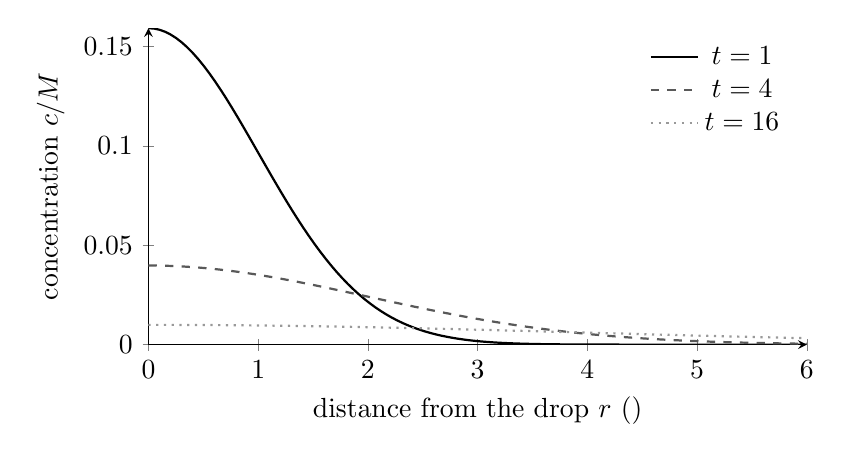
\begin{tikzpicture}
    \begin{axis}[
        width=0.82\linewidth, height=5.6cm,
        xlabel={distance from the drop $r$ (\si{\milli\metre})},
        ylabel={concentration $c / M$},
        xmin=0, xmax=6, ymin=0,
        domain=0:6, samples=120,
        axis lines=left, legend style={draw=none},
        scaled y ticks=false,
        yticklabel style={/pgf/number format/fixed},
        cycle list={{black, thick}, {black!65, thick, dashed},
                    {black!40, thick, dotted}},
      ]
      \addplot {exp(-x^2/(4*0.5*1))/(4*pi*0.5*1)};
      \addlegendentry{$t = \SI{1}{\second}$}
      \addplot {exp(-x^2/(4*0.5*4))/(4*pi*0.5*4)};
      \addlegendentry{$t = \SI{4}{\second}$}
      \addplot {exp(-x^2/(4*0.5*16))/(4*pi*0.5*16)};
      \addlegendentry{$t = \SI{16}{\second}$}
    \end{axis}
  \end{tikzpicture}
  \caption{Pigment concentration across the stain, from~\eqref{eq:solution}.}
  \label{fig:profiles}
\end{figure}

Different papers spread ink by different amounts, mostly
because their fibres leave channels of different sizes.
Table~\ref{tab:papers} lists illustrative values for three
common fibres.

\begin{table}[h]
  \centering
  \begin{tabular}{l l S[table-format=1.1]}
    \toprule
    Paper & Fibre & {Spread after \SI{10}{\second} (\si{\milli\metre})} \\
    \midrule
    Kozo      & long, coarse & 6.5 \\
    Mitsumata & fine, soft   & 4.0 \\
    Gampi     & very fine    & 2.5 \\
    \bottomrule
  \end{tabular}
  \caption{Illustrative spread for three washi fibres. The values are
    made up for this example.}
  \label{tab:papers}
\end{table}
